% Declaring packages and formatting
\documentclass[a4paper]{article}

\usepackage{graphicx} % EFor graphics
\usepackage{amsmath} % For mathematics
\usepackage{setspace} % For doublespacing
\usepackage{fancyhdr} % For headers
\usepackage{siunitx} % For SI units
\usepackage[scale=0.75]{geometry} % For wider pages
\usepackage[colorlinks = true, urlcolor = blue, linkcolor = black]{hyperref} % For hyperlinks


% Let's begin the document
\begin{document}
	% Let's set up our headers, footers and doublespacing
	\pagestyle{fancy}
	\renewcommand{\headrulewidth}{0pt}
	\renewcommand{\footrulewidth}{0.4pt}
	\renewcommand{\subsectionmark}[1]{}
	\renewcommand{\sectionmark}[1]{\markboth{#1}{}}
	\cfoot{Last Updated -- \today \\ Tim Snow -- \href{http://www.cunninglemon.com}{http://www.cunninglemon.com} \\ \vspace{1em} 
\includegraphics[height=2em]{Graphics/License}}
	\rfoot{\thepage}
	\doublespacing

	\begin{centering}
 		\section*{pH Calculator}
 		\label{sec:ph_calculator}
	\end{centering} 	

		\begin{figure}[ht!]
			\centering
			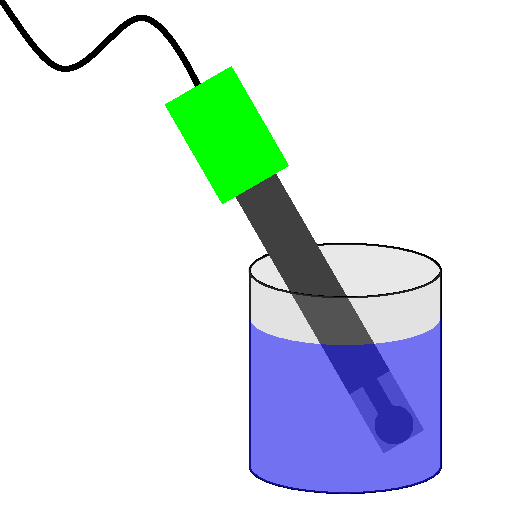
\includegraphics[height=6em]{Graphics/phIcon}
		\end{figure}

		\noindent This program has been designed to be small and simple, it calculates the concentration of [H]$^{+}$ or [OH]$^{-}$ ions in the pH adjustor you are using and the concentration in your current sample solution and informs you how much of the adjustor would be required to adjust the sample to a particular pH. As it is anticipated that a highly concentrated adjustor will be used effects due to dilution are ignored, as are any buffering properties that the sample solution may posses, however these both of these factors are working for you as it is always easier to add more adjustor than to neutralise it.

		\begin{equation}
			\text{[H]}^{+} = 10^{-\text{pH}} \quad \text{or} \quad \text{[OH]}^{-} = 10^{-(14-\text{pH})}
			\label{eq:hPlusIons}
		\end{equation}

		\noindent Using equation \ref{eq:hPlusIons} the number of [H]$^{+}$ or [OH]$^{-}$ present in both the adjustor and sample can quickly be determined, as well as the target ion concentration. From here simply subtracting the target ion concentration from the current ion concentration, divided by the adjustor ion concentration will reveal the ratio required. Multiplying this by the sample volume and subsequently by a thousand, to convert from \si{\milli\liter} to \si{\micro\liter}, it is possible to work out the required volume of adjustor to change the sample pH to the desired pH, as outlined in equation \ref{eq:adjustorVolume}. Naturally, [H]$^{+}$ can be substituted for [OH]$^{-}$ in equations \ref{eq:adjustorVolume} and \ref{eq:neutralisation}.

		\begin{equation}
			\text{Adjustor Volume} = \left( \frac{\text{[H]}^{+}_{\text{Target}} - \text{[H]}^{+}_{\text{Current}}}{\text{[H]}^{+}_{\text{Adjustor}}} \right) \times \text{Volume} \times 1000
			\label{eq:adjustorVolume}
		\end{equation}

		\noindent As one might imagine, if neutralisation should be required before the adjustment shown in equation \ref{eq:adjustorVolume} this will increase the amount of adjustor required. This can be determined by equation \ref{eq:neutralisation} and the program will, depending on the numbers input, work out whether only neutralisation is required or whether neutralisation is required in addition to further alteration of the pH. For full details on how this is implemented review the program comments in the source code.

		\begin{equation}
			\text{Adjustor Volume} = \left( \frac{\text{[H]}^{+}_{\text{Target}} + \text{[OH]}^{-}_{\text{Neutralisation}}}{\text{[H]}^{+}_{\text{Adjustor}}} \right) \times \text{Volume} \times 1000
			\label{eq:neutralisation}
		\end{equation}

		\clearpage

		\begin{figure}[ht!]
			\centering
			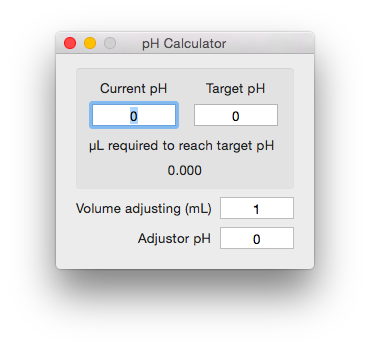
\includegraphics[width=0.4\textwidth]{Graphics/ScreenOne} 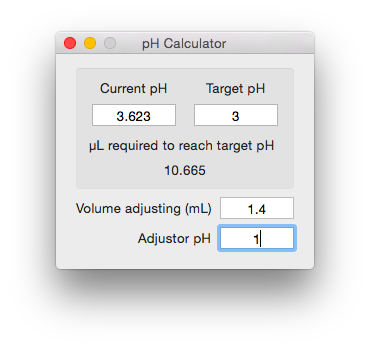
\includegraphics[width=0.4\textwidth]{Graphics/ScreenTwo}
		\end{figure}


		\noindent The figure on the left shows the program startup screen. Simply entering numbers, as shown on the figure on the right, will provide the volume of adjustor, in \si{\micro\liter}, required to change the given volume of sample solution, in \si{\milli\liter}, depending on parameters entered by the user. The numbers given here can also be scaled by thousands, \textit{e.g.} the volume, in \si{\milli\liter}, required to adjust the pH of a sample, in \si{\liter}.

		\clearpage


	\begin{centering}
 		\section*{Requirements and License}
 		\label{sec:requirements_and_license}
	\end{centering} 
		
			\noindent This software should work work with any Macintosh computer running Mac OS 10.10 or later and is released under the BSD 3-Clause license, as follows:

			\begin{figure}[ht!]
				\centering
				
\includegraphics[height=6em]{Graphics/BSD}
			\end{figure}

			\begin{quote}
				{\it
					Copyright \textcopyright 2015, Tim Snow\\
					All rights reserved.

					Redistribution and use in source and binary forms, with or without modification, are permitted provided that the following conditions are met:

					1. Redistributions of source code must retain the copyright notice, this list of conditions and the following disclaimer.\\
					2. Redistributions in binary form must reproduce the copyright notice, this list of conditions and the disclaimer found in the license file and/or other materials provided with the distribution.\\
					3. Neither authors' names of its contributors may be used to endorse or promote products derived from this software without specific prior written permission.

					THIS SOFTWARE IS PROVIDED BY THE COPYRIGHT HOLDERS AND CONTRIBUTORS "AS IS" AND ANY EXPRESS OR IMPLIED WARRANTIES, INCLUDING, BUT NOT LIMITED TO, THE IMPLIED WARRANTIES OF MERCHANTABILITY AND FITNESS FOR A PARTICULAR PURPOSE ARE DISCLAIMED. IN NO EVENT SHALL THE COPYRIGHT HOLDER OR CONTRIBUTORS BE LIABLE FOR ANY DIRECT, INDIRECT, INCIDENTAL, SPECIAL, EXEMPLARY, OR CONSEQUENTIAL DAMAGES (INCLUDING, BUT NOT LIMITED TO, PROCUREMENT OF SUBSTITUTE GOODS OR SERVICES; LOSS OF USE, DATA, OR PROFITS; OR BUSINESS INTERRUPTION) HOWEVER CAUSED AND ON ANY THEORY OF LIABILITY, WHETHER IN CONTRACT, STRICT LIABILITY, OR TORT (INCLUDING NEGLIGENCE OR OTHERWISE) ARISING IN ANY WAY OUT OF THE USE OF THIS SOFTWARE, EVEN IF ADVISED OF THE POSSIBILITY OF SUCH DAMAGE.
				}
			\end{quote}
\end{document}